% !TeX TS-program = txs:///duck
\documentclass{standalone}
\usepackage{tikzducks}
\usepackage{marvosym}

\definecolor{sgskin}{RGB}{222,197,159}
\definecolor{sgblond}{RGB}{238,203,96}
\colorlet{sggreen}{olive!50!black}
\colorlet{sgbill}{sgskin!85!black}
\colorlet{sgshirt}{sggreen!50!black}

\begin{document}
	

\begin{tikzpicture}
	\duck[
		body=sgskin,
		bill=sgbill,
		tshirt=sgshirt,
		jacket=sggreen,
		cap=sggreen
	]
\end{tikzpicture}


\begin{tikzpicture}
	\duck[
		body=sgskin,
		bill=sgbill,
		tshirt=sgshirt,
		jacket=sggreen,
		shorthair=sgblond
	]
\end{tikzpicture}


\begin{tikzpicture}
	\duck[
		body=sgskin,
		bill=sgbill,
		tshirt=sgshirt,
		jacket=sggreen,
		parting=brown!70!black,
		glasses=brown!30!gray, 
		book={\AA}, 
		bookcolour=brown!50!black
	]
\end{tikzpicture}

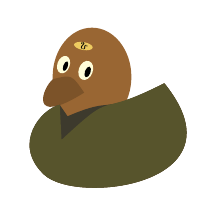
\begin{tikzpicture}
	\duck[
		body=brown!80!black,
		bill=brown!65!black,
		tshirt=sgshirt,
		jacket=sggreen,
		grumpy
	]
	\fill[sgblond, rotate=-10] (0.45,2.0) ellipse (0.12 and 0.05);
	\node[rotate=170] at (0.8,1.89) {\scalebox{0.35}{\Leo}};
\end{tikzpicture}
	
\end{document}